%!TEX TS-program = arara
%!TEX encoding = UTF-8 Unicode
% copyright dokenzy@gmail.com
% 
% arara: xelatex: {shell: yes}
%
\documentclass[oneside, chapter, 11pt]{oblivoir}

\usepackage{ccicons}
\usepackage{etoolbox}
\usepackage{graphicx}
\graphicspath{{images/}}
\usepackage{kotex-logo}
\newcounter{hindex}
\setcounter{hindex}{2}

\usepackage{makeidx}
\makeindex

\usepackage{tabu}
\usepackage{paralist}
\usepackage[dvipsnames, svgnames, x11names]{xcolor}
\definecolor{SunOrange}{cmyk}{0,.47,.78,0}

\usepackage[most]{tcolorbox}
\tcbuselibrary{minted}



\hypersetup{
	pdfauthor={dokenzy},
    pdftitle={모두를 위한 LaTeX},
    pdfsubject={LaTeX을 시작하려는 사람들을 위한 성의없는 설명서},
    pdfkeywords={LaTeX, 매뉴얼, 너무 성의없다},
    colorlinks= true,
    linkcolor=blue,
    urlcolor=blue,
    citecolor=blue,
    anchorcolor=blue
}
\newcommand{\inlinecode}[1]{\raisebox{0.25ex}{#1}}
\newcommand{\google}{구글}
\newcommand{\texworks}{TeXworks}

\setlength\parskip{1.0em}
\setlength\parindent{0pt}

% 예제결과 박스
\newmdenv[%
	nobreak=true,
	roundcorner=5pt,
	linewidth=0.3pt,
	linecolor=Goldenrod,
	subtitlebelowline=true,
	subtitleaboveline=true,
	backgroundcolor=white, 
	frametitle=결과,
	frametitlefont=\ttfamily\small,
	frametitlerule=true, 
	frametitlerulewidth=0.5pt,
	frametitlebackgroundcolor=Gold
]{showresult}

% 예제코드 박스
\mdtheorem[%
	nobreak=true,
	linewidth=0.3pt ,%
	innerleftmargin=5pt,
	innerrightmargin=5pt,
	innertopmargin=15pt,
	innerbottommargin=3pt,
	leftmargin = 40 ,%
	rightmargin = 40 ,%
	leftmargin=0em,
	rightmargin=0em,
	linecolor=Goldenrod,
	roundcorner=5pt,
	backgroundcolor=Cornsilk1,
	frametitlerule=true,%
	frametitlebackgroundcolor=Gold,
	frametitlefont=\sffamily\small,
	frametitleaboveskip=2pt,
	frametitlebelowskip=2pt]
{mdcodebox}{Code}

\BeforeBeginEnvironment{pyglist}{\begin{mdcodebox}}
\AfterEndEnvironment{pyglist}{\end{mdcodebox}}

% 그림 캡션 모양
\captiondelim{ } % "그림:" 에서 ":"을 없앰
\captionnamefont{\footnotesize\bfseries\sffamily} % "그림"을 굵게
\captiontitlefont{\footnotesize\sffamily} % 본문은 보통 굵기로

%\setmonofont{NanumBarunGothicOTF}
\setmainhangulfont{HCR Batang LVT}
\setsanshangulfont{HCR Dotum LVT}
\setmonohangulfont[Scale=.9]{HCR Dotum LVT}
\newfontface{\applesymbol}{Apple Symbols}
\newfontface{\zapfino}{Zapfino}



\newcommand{\version}{0.6.5}
\title{모두를 위한 \LaTeX\\\small{부제: 근본없는 매뉴얼}}
\author{dokenzy@gmail.com\\nova de hi}
\date{\version판\\2015년 6월 12일}
\feetbelowfloat

\begin{document}
\maketitle
\begin{abstract}
이 문서의 목적은 대략적인 \LaTeX 문서작성방법을 소개하고, 좋은 \LaTeX 설명서를 소개하는 것이다. 이 문서를 읽고 \LaTeX을 제대로 배우고 싶은 분들은 이 문서 마지막에 있는 \ref{chap:docs}\chaptername~\titleref{chap:docs}\을 읽기를 바란다.
\end{abstract}

\begin{center}
\ccbyncsa\\
{\scriptsize 이 저작물은 크리에이티브 커먼즈 저작자표시 4.0 국제 라이선스\footnote{\href{http://creativecommons.org/licenses/by/4.0/}{http://creativecommons.org/licenses/by/4.0/}}에 따라 이용할 수 있습니다.}
\end{center}

\clearpage
\section*{바뀐 점}
\begin{description}
\item[\version] 2015년 6월 12일. 코드환경을 tcolorbox와 minted 조합으로 변경(nova de hi님)
\item[0.6] 2014년 3월 25일. 특수문자 설명 추가, 참고문헌 추가, 자잘한 부분 수정
\item[0.5] 2014년 2월 18일. TeX Live 업데이트 내용 추가, 자잘한 부분 수정
\item[0.4] 2014년 2월 4일. 찾아보기 추가, defaultfontfeatures 내용 추가, 카운터 이름 변경, 추천문서 추가, 자잘한 것 몇 개 수정
\item[0.3] 2013년 12월 20일. 맞춤법 수정, MWE 내용 추가, 자잘한 것 몇 개 수정. 조언해주신 이주호님께 감사드립니다.
\item[0.2] 2013년 12월 20일. `워드 프로세서, 멍청하고 비효율적인 도구' 한글판 링크 추가, 자잘한 것 몇 개 수정
\item[0.1] 2013년 12월 13일. 최초 공개
\end{description}
\clearpage

\tableofcontents
%\listoffigures
%\listoftables

\frontmatter
\chapter{들어가며}
\section{왜 \LaTeX인가?}
이 문서는 나 자신이 \LaTeX\footnote{레이텍 또는 라텍이라 읽는다.}을 하며 느꼈던 점들을 바탕으로 만든 \LaTeX초보용 문서이다. 나는 \LaTeX뿐만 아니라 조판 및 인쇄 전반에 대한 실무경험이 전혀 없을 뿐 더러, 이론적 지식도 영화 `그라비티'에 나오는 사람 수만큼 밖에 안된다. 맞춤법도 그다지 자신 없다. 다만, 마크업과 일반 텍스트(plain text)를 동경하는 사람으로서 최소한의 노력으로 최대한 멋진 문서를 만들고 싶은 욕심이 있다. 

나처럼 마크업과 일반 텍스트를 이용해서 문서를 만드는 사람이 많을 것이다. Markdown이나 reStructuredText 같은 것들이 개발자들에게 많이 쓰이는 이유이기도 하다. Markdown이나 reST가 생산적으로 문서를 만들어 주긴 하지만 멋진 문서를 만들어 주지는 않는다. 이를 충족시킬 수 있는 도구가 \LaTeX이다. 매크로 언어인 \LaTeX과 조판프로그램인 \TeX을 이용하면 생산적이면서도 품위있는 문서를 만들 수 있다. 

워드프로세서와 무엇이 어떻게 다른지 궁금한 사람들을 위해 \href{http://nitens.org/taraborelli/latex}{The Beauty of \LaTeX}이라는 글을 소개한다. 해석하지 않아도 된다. 단지 눈으로 비교해 보는 것만으로도 충분하다. 게다가 워드프로세서는 물론, 인디자인 같은 전문 조판 프로그램조차 상상도 할 수 없는 일을 할 수 있다. 2011년 한국텍학회 학술대회에서 조진환 교수님께서 발표하신 \index{함초롬}\href{http://conf.ktug.org/2011/Program_files/KTS2011-chof.pdf}{함초롬 - 글꼴을 이용한 자소 분리}를 보라(\figurename~\ref{fig:hcr}). 이 발표는 2013년 10월에 열린 \href{http://tug.org/tug2013/}{TUG 2013}에서도 발표되어 큰 관심을 받았다.

CSS 없이 HTML 코드에 스타일을 구겨 넣었던 1990년대를 기억하는가? 그런데 워드프로세서는 왜 아직도 그 꼴을 벗어나지 못하는 것인가? 워드프로세서는 할 수 없다. 앞으로도 그렇다. 김강수님이 번역하신 \href{https://www.dropbox.com/s/fjmszvq6f05dlxg/wpkor.pdf}{워드 프로세서, 멍청하고 비효율적인 도구}라는 글을 읽어보자. 나 또한 완전히 동의한다. 이제 워드프로세서의 늪에서 벗어나 보자.

\begin{figure}[!hbtp]
\caption{함초롬을 이용한 자소 분리(조진환)}
\label{fig:hcr}
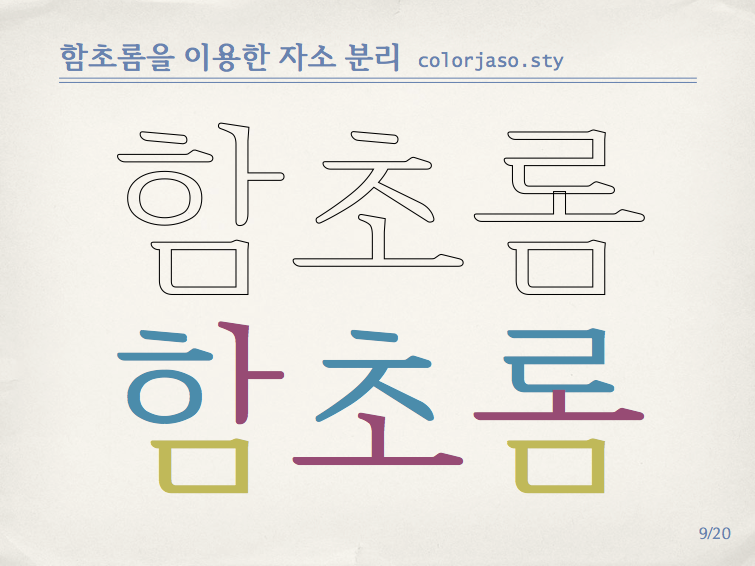
\includegraphics[width=\textwidth]{KTS2011-chof}
\end{figure}

\section{한국텍학회와 한글텍사용자그룹}\label{sec:ktug}
\index{한국텍학회}\index{한글텍사용자그룹}
내가 이 문서를 만들 수 있게 된 것은 한국텍학회(KTS)\footnote{\href{http://www.ktug.org/xe/?mid=KTS}{The Korean TeX Society}}와 한글\TeX사용자그룹(KTUG)\footnote{\href{http://ktug.org}{http://ktug.org}}에서 활동하시는 몇몇 분들의 헌신적인 노력 덕분이다. 이분들은 \koTeX\footnote{`케이오텍' 또는 `코리언 텍'이라고 읽는다.}을 개발하셨을 뿐만 아니라 관련 문서들을 직접 쓰거나 번역하시고 정기적인 워크숍 등을 통해 무료로 교육까지 하신다. 그뿐만 아니라 TnX텍 같은 유용한 유틸리티 프로그램도 개발하셨다. 내가 \LaTeX을 배울 수 있었던 것은 모두 이분들의 공헌 덕분이다. 이분들은 \TeX 뿐만 아니라 타이포그래피, 레이아웃, 배치(batch)처리, 폰트 등 조판과 인쇄분야 전반에 해박한 지식과 풍부한 경험이 있다. 위에서 보인 `\titleref{fig:hcr}'(\figurename~\ref{fig:hcr})에 쓰인 폰트는 `한글과컴퓨터'사에서 개발한 함초롬폰트에 한국텍학회가 GSUB/GPOS 정보를 추가하여 재배포하는 폰트\label{hcr}다.\footnote{이 폰트에 대한 자세한 정보는 \href{http://wiki.ktug.org/wiki/wiki.php/\%ED\%95\%A8\%EC\%B4\%88\%EB\%A1\%AC\%EC\%B2\%B4LVT}{함초롬체LVT}를 참고하라.}

2013년 11월 9일, 한국어 조판을 위한 \koTeX이 TeXLive 2013에 드디어 정식으로 포함되었다. 이것은 당신이 만든 Python 라이브러리가 Python 표준 라이브러리에 등록된 것과 비슷하다. 물론 TeXLive에 포함되기 전에도 \koTeX으로 한국어 문서를 조판할 수 있었지만, 이젠 TeXLive에 포함됨으로써 별도의 설치과정을 거치지 않아도 된다.
% wordprocessor.pdf translated by Karnes

\section{\XeLaTeX은 무엇인가?}
\index{XeLaTeX}
이 \sectionname에서 언급하는 단어들을 처음 접하는 사람들은 혼란스러울 수 있다. 아니면 이미 등장한 \LaTeX, \koTeX, \TeX이란 용어때문에 아까부터 혼란스러운 사람이 있을 수도 있다. 조금이라도 혼란스럽다면 과감히 이 \sectionname을 넘어가자. 시작하기도 전에 용어 때문에 스트레스받지 말자. 자동차 운전을 처음 배우는 사람이 자동차 엔진부터 배울 필요는 없다. 이 문서는 운전을 시연하는 수준일 뿐이다. \LaTeX이라는 차를 어떻게 운전하는지 지켜본다는 마음으로 가볍게 읽자.

\LaTeX은 매크로언어이다. \LaTeX을 한다는 말은 이 매크로언어로 만든 텍 파일(*.tex)을 처리해서 최종적으로 원하는 문서(예를 들면, PDF파일)를 만든다는 것이다. 이 텍 파일을 처리하기 위해서는 텍 엔진이라는 프로그램이 필요하다. 현재 TeXLive에는 5개의 텍 엔진이 있는데 이 문서에서는 \XeTeX이라는 엔진을 이용한 방법만 다룬다. \XeTeX은 시스템에 설치된 대부분의 truetype이나 opentype 폰트 등을 직접 사용할 수 있기 때문이다.\footnote{\XeTeX에서 사용하지 못하는 트루타입이나 오픈타입 폰트는 대부분 폰트 자체에 문제가 있다.}

\koTeX은 \TeX으로 한글을 조판하기 위한 시스템이다. \XeTeX-\ko는 \XeTeX 엔진을 위한 \koTeX 패키지이다. \koTeX 2.0 설명서에 따르면 현재 한글 문헌을 가장 안정적으로 조판할 수 있는 것은 \XeTeX-\ko라고 한다. 그래서 이 문서에서는 \XeLaTeX만을 다룬다.\footnote{내가 그나마 조금 할 줄 아는 것도 이것 뿐이다.} \XeLaTeX이란 `\XeTeX이라는 텍 엔진'으로 `\LaTeX 매크로언어로 작성한 텍 파일'을 처리하는 프로그램이라고 할 수 있겠다.

\mainmatter
\chapter{첫걸음}
\section{운영체제별 설치}
\index{설치}
\LaTeX을 사용하기 위해서는 TeXLive 2013을 설치해야 한다.\footnote{\href{http://www.tug.org/texlive/}{http://www.tug.org/texlive/}} TeXLive는 사실상의 표준 텍 시스템으로서 Mac OS X, 윈도우즈, 리눅스 운영체제에서 사용할 수 있다. 텍 시스템은 많은 유틸리티와 방대한 라이브러리, 스타일, 폰트 등으로 구성된 큰 시스템이다. MacTeX의 경우 설치파일만 2.3GB에 달한다. 전문가는 원하는 부분만 설치해서 사용하는 것도 가능하지만, 이 문서에서는 텍 시스템 전체를 설치하는 것만 다룬다.

\begin{description}
\item[Mac] MacTeX 2013\footnote{\href{http://tug.org/mactex/}{http://tug.org/mactex/}}을 설치한다. 이 배포판은 Mac 10.5(Leopard) 이상에서 사용할 수 있다. 인스톨러의 안내대로 설치하면 끝난다.
\item[Windows] 윈도우즈 사용자는 KTS와 KTUG에서 제작한 ko.TeXLive 2013\footnote{\href{http://www.ktug.org/xe/index.php?mid=KTUG_open_board&document_srl=175806}{ko.TeX Live 2013}}을 이용하면 쉽게 설치할 수 있다. 인스톨러의 안내대로 설치하면 끝난다. 설치 중 일부 파일에 대해 백신 프로그램이 바이러스로 오진하여 설치가 중단될 수 있다. 이럴 때는 잠시 백신을 중지하고 설치하자.
\item[Linux] 리눅스에서는 인터넷을 통해 설치하는 방법을 추천한다. 설치페이지에서 install-tl-unx.tar.gz파일을 다운로드한 후 install-tl 설치 스크립트를 이용해서 설치한다. perl-tk가 설치되어 있다면 설치 스크립트를 실행할 때 -{}-gui 옵션을 추가하여 GUI로 설치를 진행할 수 있다. 일부 배포판의 경우 개인 사용자들이 패키징을 해놓은 것들이 있다. 이런 패키지를 이용하는 방법도 있다.
\end{description}

\paragraph{TeXLive 업데이트}
MacTeX이나 ko.TeXLive 2013으로 설치한 후에는 업데이트를 해주어야 한다. 또한 TeXLive를 사용하다가도 한 달에 한 번 정도는 업데이트를 해주는 것이 좋다. TeX Live를 최신 버전으로 업데이트하기 위해서는 명령행에서 다음 명령을 실행한다.

\begin{pyglist}[language=bash]
$ tlmgr update --self --all
\end{pyglist}

위 명령을 실행했는데 퍼미션 오류가 발생한다면 root권한으로 위 명령을 실행해야 한다. Mac OS X나 데비안 계열의 경우 sudo와 함께 사용하면 된다. 다른 리눅스에서도 root권한으로 실행하면 된다.

업데이트를 오랫동안 안하면 \figurename~\ref{fig:update}처럼 수백 개를 한 번에 업데이트하게 되는 수가 있다.
\begin{figure}
\caption{tlmgr update}
\label{fig:update}
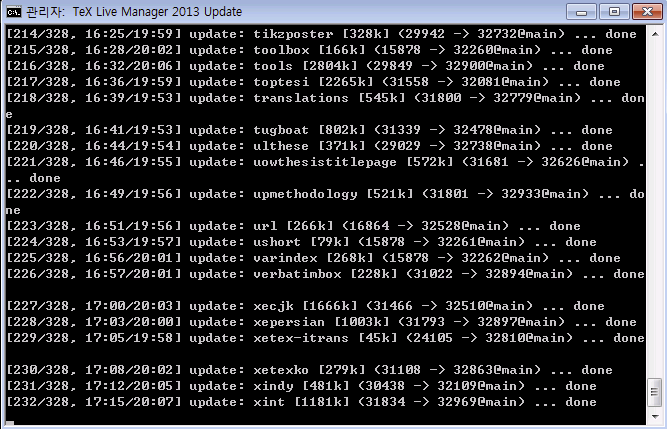
\includegraphics[width=\textwidth]{tlmgr-update}
\end{figure}

\section{Mac OS X에서 폰트경로 설정하기}
Mac OS에서는 \XeTeX을 위한 설정을 한 번 해주어야 한다. \footnote{윈도우즈는 \texttt{fc-cache}명령을 실행해야 한다. ko.TeX Live 2013는 설치 과정 마지막에 자동으로 해준다. 하지만 설치 후에 추가된 폰트를 사용하기 위해서는 이 명령을 직접 실행해 주어야 한다.}

/usr/local/texlive/2013/texmf.cnf 파일을 텍스트 에디터로 열어서 다음 내용을 추가하자.

\begin{pyglist}[language=bash]
OSFONTDIR = {~/Library/Fonts;/Library/Fonts;/System/Library/Fonts}
\end{pyglist}

이 설정을 하면 시스템 라이브러리나 사용자 라이브러리 폴더에 있는 폰트들을 \XeTeX이 사용할 수 있다. 
자세한 내용은 \href{http://wiki.ktug.org/wiki/wiki.php/MacOSInstall}{KTUG wiki}를 참고하자.

그리고 블로그 `도은이네 집'에서 소개한 \href{http://doeun.tistory.com/172}{맥 오에스 폰트 라이브러리 등록} 글에 소개된 내용도 적용하자. TeXLive를 설치하면 많은 폰트들이 함께 설치되는데, 이 경로는 위에서 설정한 경로와 다르다. \XeTeX이 이 폰트들을 사용하기 위한 방법이다.
\begin{enumerate}
\item 서체 관리자(Font Book)을 실행한다.
\item 파일-새로운 보관함(New Library) 메뉴를 선택하고 `TL OpenTypes'라고 이름을 지어주자.
\item 방금 만든 `TL OpenTypes'를 오른쪽 클릭하여 `서체 추가...'를 선택하자.
\item 파일 선택창이 열리면 `{\applesymbol ⇧+⌘+}G'키를 눌러 경로창을 띄운 후 다음 주소를 입력하자.
\begin{pyglist}
/usr/local/texlive/2013/texmf-dist/fonts/opentype/public
\end{pyglist}
굉장히 많은 폰트들이 각 폴더에 들어있다. 전부 다 해도 되고 원하는 폰트(폴더)만 선택해도 된다.
\end{enumerate}
같은 방식으로 truetype 폰트들도 추가할 수 있다.\footnote{/usr/local/texlive/2013/texmf-dist/fonts/truetype/public} 이제 Mac에서 \XeTeX을 사용하기 위한 설정을 모두 마쳤다\footnote{윈도우즈에서는 폰트를 시스템에 설치할 때마다 fc-cache 명령을 실행하면 된다.}.

\section{테스트}\label{sec:test}
이제 \LaTeX을 사용하기 위한 준비를 모두 마쳤다. 아무 텍스트 편집기라도 사용할 수 있지만 여기서는 TeXLive를 설치할 때 함께 설치되는 \texworks를 사용하기로 한다. \texworks를 실행하고 아래 코드를 입력하자.

\begin{pyglist}
\documentclass[oneside, a4paper]{article}
\usepackage{kotex}
\setmainhangulfont{HCR Batang LVT}
% 함초롬 바탕 LVT를 다운로드 & 설치하자
% 다운로드 주소: http://bit.ly/1hnXefL
\begin{document}
\section[시작]{\LaTeX 시작하기}
\begin{center}
안녕, \LaTeX!
\end{center}
한 번 배워서 오래 써먹자.
\end{document}
\end{pyglist}

입력을 마치면 foo.tex이라는 이름으로 저장하자.

이제 텍 엔진을 \figurename~\ref{fig:TeXworksButton}\과 같이 선택하고 컴파일 버튼을 누르거나 [조판] 메뉴에서 `조판'을 누르자. 또는 단축키를 이용할 수도 있다.
\begin{figure}[!hbp]
\caption{TeXworks의 컴파일 버튼과 텍 엔진}
\label{fig:TeXworksButton}
\begin{center}
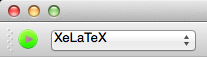
\includegraphics[scale=0.7]{TeXworksButton}
\end{center}
\end{figure}

\begin{inparaenum}[1)]
\item TeXLive 2013이 제대로 설치되고, \item 소스코드에 오류가 없고, \item 텍 엔진을 올바르게 선택했다면
\end{inparaenum} 컴파일이 끝난후, 화면 오른쪽에 \figurename~\ref{fig:foo}처럼 foo.pdf 파일이 보일 것이다.

\begin{figure}[!hbtp]
\caption{foo.pdf}
\label{fig:foo}
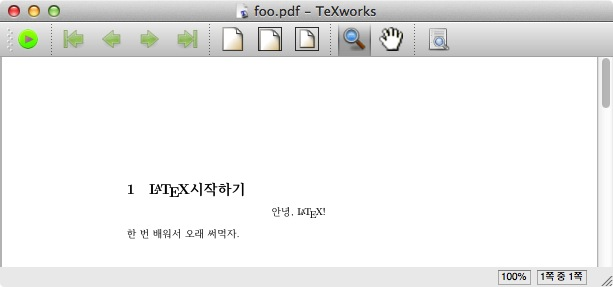
\includegraphics[width=\textwidth]{foo}
\end{figure}
나는 Skim\footnote{\href{http://skim-app.sourceforge.net/}{http://skim-app.sourceforge.net/}}이라는 PDF리더를 주로 사용하지만, PDF파일의 정보를 볼 때는 Adobe사의 Acrobat Reader를 사용하기도 한다. Acrobat Reader로 foo.pdf파일의 속성을 보면 \figurename~\ref{fig:fooproperty}처럼 나온다. \XeTeX으로 만들었다는 것을 알 수 있다.
\begin{figure}[!htbp]
\centering
\caption{Adobe Reader로 본 문서 속성}
\label{fig:fooproperty}
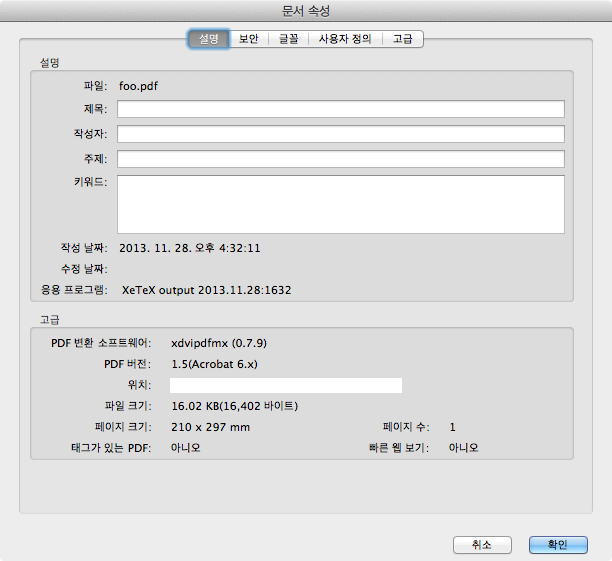
\includegraphics[width=\textwidth]{fooproperty}
\end{figure}

\section{알고보면 사연이 많은 예제코드}
\TeX은 강력한 조판시스템이다. 강력한 만큼 배울 게 많다. 앞의 예제코드는 매우 간단한 코드이지만 그 속에는 많은 사연이 들어있다. 본격적으로 시작하기 전에 예제코드를 꼼꼼히 살펴보겠다.

\subsection{클래스(documentclass)}
\index{클래스}
\index{documentclass}
예제코드의 \verb|\documentclass[oneside]{article}|부분이다.
클래스는 문서의 성격을 결정하는 가장 중요한 부분으로 tex문서를 작성할 때 반드시 가장 먼저 한 번만 쓰인다. 템플릿처럼 문서 전체의 모양을 결정할 뿐만 아니라, 많은 기능과 옵션을 제공한다. 예컨대 예제코드의 \verb|\section{시작하기}| 명령은 article 클래스가 제공하기 때문에 사용할 수 있다. 하지만 \verb|\chapter{시작하기}|명령을 사용하면 오류가 발생한다. article 클래스에는 없는 명령이기 때문이다. 또다른 표준클래스인 report 클래스는 \verb|\chapter{}|명령을 제공하기 때문에 사용할 수 있다.

oneside 옵션은 article 클래스가 제공하는 옵션이다. 이 외에 a4paper, 11pt, landscape 등의 옵션들이 있다. 어떤 옵션을 쓸 수 있는지는 전적으로 클래스에 달려있다. 만약 클래스에서 제공하지 않는 기능들을 사용하고 싶다면, 관련 패키지를 사용하거나 직접 정의(\ref{sec:newcommand}\chaptername~\titleref{sec:newcommand})해야 한다.
%
\subsection{명령(command)}\label{subsec:command}
\index{명령}
\index{command}
명령은 대체로 다음과 같은 형식을 갖는다.
\begin{pyglist}
\section[시작]{\LaTeX 시작하기}
\end{pyglist}

대괄호(\verb|[]|)는 옵션이고, 중괄호(\verb|{}|)는 명령의 이름이다. 명령에 따라 옵션이 있을 수도 있고 없을 수도 있다. 또 옵션이나 인자가 2개 이상인 명령도 있다. 만약 텍 문서를 컴파일 하는 중에 \texttt{! Undefined control sequence.} 오류가 발생한다면, 명령에 오타가 있거나 정의되지 않은 명령(클래스나 사용하는 패키지에 없는 명령)을 쓴 것이다. 이럴 때는 해당 명령을 제공하는 클래스나 패키지 매뉴얼을 읽어봐야 한다. 매뉴얼에 대한 설명은 \ref{sec:texdoc}\sectionname~\titleref{sec:texdoc}을 참조하기 바란다.

\subsection{환경(environment)}\label{subsec:environment}
환경은 \verb|\begin{center}|\ldots\verb|\end{center}|와 같은 형식을 갖는다. 옵션의 위치는 환경에 따라 조금씩 다를 수 있다.

\verb|\begin{document}|\ldots\verb|\end{document}|도 환경이다. \texttt{document} 환경은 \LaTeX 문서라면 반드시 하나만 존재해야 하는 중요한 환경이다. 마치 HTML의 \verb|<body>|태그와 같다. 환경 역시 정확한 사용방법은 매뉴얼을 보는 것이다. 

\subsection{프리앰블(Preamble)}
\index{프리앰블}
\index{Preamble}
프리앰블\footnote{전처리부라고 부를 수도 있지만, 나는 프리앰블이 익숙하다.}은 \verb|\documentclass{}|와 \verb|\begin{document}| 사이에 있는 부분을 말한다. 예제코드에서 
\begin{pyglist}
\usepackage{kotex}
\setmainhangulfont{HCR Batang LVT}
\end{pyglist}
가 위치한 곳이 바로 프리앰블이다. HTML의 \verb|<head>|태그와 비슷한 기능을 하지만 프리앰블이라고 명시하는 명령은 따로 없다. 패키지를 불러오거나(\verb|\usepackage{}|), 명령이나 환경을 정의할 때에는 프리앰블에 해야 한다.

\subsection{패키지(package)}
\index{패키지}
\index{package}
패키지를 사용하면 클래스가 제공하지 않는 많은 기능들을 이용할 수 있다. 대표적으로 한국어를 조판하기 위해서는 \koTeX 패키지를 사용해야 한다. 패키지를 사용하는 방법은 프리앰블에서 \verb|\usepackage[옵션]{패키지이름}|과 같은 방식으로 사용한다. 간혹 패키지끼리 충돌을 일으키거나 읽어들이는 순서(\verb|\usepackage{}|명령을 선언한 순서)에 따라 문제가 생길 수 있다. 이런 경우에는 \textbf{알아서 잘}(\ref{chap:mme}\chaptername~\titleref{chap:mme}) 해결하라.

\subsection{공백문자와 문단}
\index{공백문자}
\index{문단}
공백문자란 스페이스, 탭 등을 가리킨다. \TeX은 이런 공백문자들을 연속으로 입력해도 하나의 스페이스로 처리한다. HTML과 같다. \textbf{한 번의 줄바꿈}(linebreak) 역시 하나의 스페이스로 처리한다.

\LaTeX으로 문서를 작성할 때 주의해야 할 점은 문장과 문단을 엄격히 구분한다는 것이다. 워드프로세서에서는 문장, 줄바꿈, 문단 등이 아무 개념없이 사용되어도 문제를 느끼지 못하지만 \LaTeX에서는 다르다. 문단을 나누기 위해서는 문장 끝에 빈 줄을 삽입하면 된다. 또는 \verb|\par|라는 명령을 사용해도 된다.
\begin{pyglist}
이것은 첫 번째 문단의 첫 번째 문장입니다.     두 번째 문장입니다.



두   번째 문단의 첫 번째 문장입니다. 공백을 많이 쓴다고 
공백이 그만큼 생기지 않습니다. 나쁜 습관입니다.
\end{pyglist}

\begin{showresult}
이것은 첫 번째 문단의 첫 번째 문장입니다.     두 번째 문장입니다.



두   번째 문단의 첫 번째 문장입니다. 공백을 많이 쓴다고 
공백이 그만큼 생기지 않습니다. 나쁜 습관입니다.
\end{showresult}

\subsection{특수문자}
\index{특수문자}
\LaTeX에서는 몇 가지 문자들을 특별한 용도로 사용한다. 따라서 문서 내에 그냥 입력하게 되면 오류가 발생하거나 의도하지 않은 결과가 나올 것이다.
\begin{pyglist}
# $ % ^ _ & \ ~ { }
\end{pyglist}
위 특수문자들을 입력하기 위해서는 사용하고 싶은 특수문자 앞에 백슬래시(\textbackslash)를 더해주면 된다. 다만 \textbackslash의 경우 \verb|\\|는 줄바꿈명령이므로, \verb|\textbackslash|명령을 사용한다.

\%는 주석(comment)을 나타내는 특수문자이다. 따라서 \LaTeX이 컴파일 할 때 무시해 버린다. HTML의 `\verb|<!-- -->|', Python의 `\verb|#|'\과 같다.

\#은 사용자 정의 명령이나 환경을 정의할 때 사용되는 기호이다. \ref{subsec:cmd_with_option}\sectionname~\titleref{subsec:cmd_with_option}을 참고한다.

\$은 수식을 조판할 때 쓰인다. \$와 \$ 사이에 수식을 넣으면 \LaTeX이 수식을 예쁘게 조판해 준다.

\begin{pyglist}
$x=\frac{-b\pm\sqrt{b^2-4ac}}{2a}$
\end{pyglist}

\begin{showresult}
$x=\frac{-b\pm\sqrt{b^2-4ac}}{2a}$
\end{showresult}

하지만 수식을 입력할 때는 \$ 기호 대신 \verb|\[, \]|를 사용하는 것을 권한다.

\begin{pyglist}
\[x=\frac{-b\pm\sqrt{b^2-4ac}}{2a}\]
\end{pyglist}

\verb|^|, \verb|_| 은 각각 수식에서 윗첨자, 아래첨자를 뜻한다. 이외 수식과 관련한 내용은 \texttt{lshort-kr}문서의 `제 3장. 수식 조판하기'를 참조하기 바란다.

\&는 표(Table)에서 다음 열로 넘어갈 때 쓰인다.

\verb|\\|는 문단을 나눌 때도 쓰이지만, 표에서는 새로운 행을 추가할 때도 쓰인다.

\verb|~|(틸데)는 줄바꿈이 안되는, 폭이 고정된 공백을 만들어준다. 만약 $\sim$을 표시하고 싶은 거라면 \verb|$sim$|를 입력한다.

\{와 \}는 굳이 설명하지 않겠다. \verb|\begin{document}|만 봐도 어디에 쓰이는지 알 수 있을 것이다.

\subsection{따옴표}
\index{따옴표}
작은따옴표나 큰따옴표를 입력해야 하는 경우가 많다. 이 때 여는 따옴표와 닫는 따옴표의 모양이 조금 다르다. \LaTeX에서는 다음과 같이 입력하면 이들 따옴표를 이쁜 따옴표\footnote{curly quotation mark}로 만들어 준다.

\begin{pyglist}
`작은 따옴표', ``큰 따옴표''
\end{pyglist}

\begin{showresult}
`작은 따옴표', ``큰 따옴표''
\end{showresult}

이것이 가능하려면 fontspec이 제공하는 다음 명령을 프리앰블에 선언해야 한다.\footnote{자세한 내용은 KTUG QnA 게시판에 두텁님이 쓰신 \href{http://www.ktug.org/xe/index.php?mid=KTUG_QnA_board&page=2&document_srl=176043}{답글}을 읽어보자.}

\begin{pyglist}
\defaultfontfeatures{Ligatures=TeX}
\end{pyglist}

여는 따옴표(grave accent, \verb|`|)는 키보드에서 숫자 1 왼쪽에 있는 키(틸데(\textasciitilde)와 같은 자리)이고, 닫는 따옴표(vertical quote, \verb|'|)는 키보드에서 엔터키 왼쪽에 있는 키(\verb|"|와 같은 자리)이다.\footnote{이 배열은 QWERTY 자판을 기준으로 한 설명이다.}

\section{texdoc}\label{sec:texdoc}
\index{texdoc}
\verb|texdoc|명령을 이용하면 설명서를 쉽게 열 수 있다. 대부분의 클래스나 패키지의 설명서는  \texttt{<texdoc 패키지이름>}과 같은 방식으로 읽을 수 있다. 예를 들어 \koTeX에 대한 설명서를 읽기 위해서는 터미널 또는 명령프롬프트에서 \texttt{texdoc kotex} 명령을 실행하면 된다. 그러면 시스템의 기본 PDF 뷰어가 실행되면서 kotexdoc.pdf 파일이 열린다.

\chapter{기본 명령과 환경}\label{chap:basic}

\section{문서제목, 저자, 날짜}\label{sec:titleauthordate}
문서를 시작할 때 문서의 제목과 저자 이름을 밝히는 것은 기본이다. 날짜도 입력하면 좋겠다. 프리앰블에  다음을 입력한다.
\begin{pyglist}
\title{근본없는 \LaTeX 설명서}
\author{Dokenzy}
\date{단기 4346년}
\end{pyglist}
만약 날짜부분을 \verb|\date{\today}|와 같이 입력하면 자동으로 오늘 날짜를 입력해준다.
그리고 나서
\begin{pyglist}
\begin{document}
\maketitle
\end{pyglist}
와 같이 \verb|\begin{document}|다음에 \verb|\maketitle| 명령을 사용하면 된다.

\section{짜임새있는 문서 만들기}
\LaTeX은 몇 가지 장절명령을 제공함으로써 논리적인 문서를 만드는 것을 도와준다.
\verb|\chapter{}|는 장(章), \verb|\section{}|은 절(節), \verb|\subsection{}|은 소절(小節)을 의미한다. 이 명령들은 문서를 논리적으로 구분해 줄 뿐만 아니라, \verb|\tableofcontents| 명령(\ref{sec:toc}\sectionname~\titleref{sec:toc})이 차례를 만들 때 단락제목, 장절번호, 페이지번호 등을 자동으로 넣어준다. 만약 장절 명령을 쓰고 싶되, 차례에는 나타내고 싶지 않다면 \verb|\chapter*{}|와 같이 \textbf{*}를 붙여주면 된다.

단락제목이 너무 길면 차례에서 볼 때 불편할 수 있다. 이 때는 \verb|\chapter[short title]{very long chapter title}|과 같이 옵션을 주면, 차례에는 `short title'이, 본문에는 `very long chapter title'이 들어간다.

\section{목록}
\index{목록}
문서를 작성하다보면 목록을 만들 필요가 있다. 이런 경우들이다.
\begin{pyglist}
\begin{itemize}
\item 좋아하는 연예인
\item 좋아하는 텍스트 편집기
\item 우리동네에 있는 카페
\end{itemize}
\end{pyglist}

\begin{showresult}
\begin{itemize}
\item 좋아하는 연예인 이름
\item 좋아하는 편집기
\item 우리동네에 있는 카페
\end{itemize}
\end{showresult}

HTML의 \verb|<ul>|태그와 같다. 항목 기호를 점 대신 하이픈(-)으로 하고 싶다면, 옵션을 넣어준다. 만약 특정 항목의 기호만 바꾸고 싶다면 해당 항목에만 옵션을 주면 된다.
\begin{pyglist}
\begin{itemize}[-]
\item 좋아하는 연예인
\item[*] 좋아하는 텍스트 편집기
\item 우리동네에 있는 카페
\end{itemize}
\end{pyglist}

\begin{showresult}
\begin{itemize}[-]
\item 좋아하는 연예인
\item[*] 좋아하는 텍스트 편집기
\item 우리동네에 있는 카페
\end{itemize}
\end{showresult}

만약 순서가 중요한 경우라면 itemize 환경 대신 enumerate\index{enumerate} 환경을 이용하자. \TeX이 알아서 번호를 매겨준다. HTML의 \verb|<ol>|태그와 같다.
\begin{pyglist}
\begin{enumerate}
\item 좋아하는 연예인 이름
\item 좋아하는 편집기
\item 우리동네에 있는 카페
\end{enumerate}
\end{pyglist}

\begin{showresult}
\begin{enumerate}
\item 좋아하는 연예인 이름
\item 좋아하는 편집기
\item 우리동네에 있는 카페
\end{enumerate}
\end{showresult}

항목 기호를 아라비아 숫자 대신 알파벳 소문자로 나타내고 싶다면\ldots? 그 방법은 이 문서에서 다루지 않는다. \google에서 검색하기 바란다. 검색 키워드는 `\href{http://goo.gl/iNsXoD}{latex enumerate numbering style}'.

\section{차례}\label{sec:toc}
\index{차례}
\index{tableofcontents}
차례없는 문서는 핸들없는 자동차와 같다. \LaTeX으로 차례를 만드는 방법은 아주 간단하다. \ref{sec:titleauthordate}\sectionname~\titleref{sec:titleauthordate}에서 설명한 \verb|\maketitle| 다음에 \verb|\tableofcontents|명령을 사용하면 된다. 

\begin{pyglist}
\begin{document}
\maketitle
\tableofcontents
\end{pyglist}

중요한 점은 최소 두 번 이상 컴파일해야 차례를 만들 수 있다. 한 번 컴파일하고 나서 PDF문서를 보면 차례에 아무 것도 나오지 않는 것을 쉽게 알 수 있을 것이다. 대신 \texttt{foo.tex} 파일과 같은 폴더에 \texttt{foo.toc} 파일이 생겼을 것이다. 왜 두 번 이상 컴파일 해야 하는지, 어떻게 자동으로 만들어지는지 궁금한 사람은 foo.toc 파일을 살펴보기 바란다.

\chaptername, \sectionname에 대한 차례 뿐만 아니라 \figurename이나 \tablename의 차례도 자동으로 만들 수 있다. 각각 다음 명령을 사용하자: \verb|\listoffigures|, \verb|listoftables|
%
\section{찾아보기(색인)}
\index{찾아보기}
\index{색인}
큰 문서의 맨 끝에는 보통 찾아보기가 온다. 찾고자 하는 내용이 어디있는지 쉽게 찾아갈 수 있는 기능을 제공한다. \LaTeX은 찾아보기도 쉽게 만들 수 있다. 이 문서에서는 \XeLaTeX에서 찾아보기를 만드는 방법만 제공한다.

먼저 프리앰블에 다음 명령을 입력한다.
\begin{pyglist}
\usepackage{makeidx}
\makeindex
\end{pyglist}

그리고 본문에서 찾아보기에 들어갈 단어를 다음과 같이 입력한다.

\begin{pyglist}
우쭈쭈\index{우쭈쭈}
\end{pyglist}

이제 찾아보기에서 우쭈쭈 항목 옆에 쪽번호를 누르면 바로 여기 `우쭈쭈'\index{우쭈쭈}로 오게 된다.

마지막으로 문서에서 찾아보기가 들어갈 곳에 \verb|\printindex| 명령을 사용한다.

이제 문서를 컴파일해서 idx 파일을 얻은 후, texindy라는 별도의 유틸리티를 사용한 후, 다시 컴파일한다. 다음과 같이 하면 된다.

\begin{pyglist}
# xelatex foo
# texindy -L korean -I omega foo.idx
# xelatex foo
\end{pyglist}

만약 차례, 상호참조 등을 사용한다면 xelatex으로 컴파일을 두 번 이상 한다. 끝이다. 이제 찾아보기 항목의 `ㅇ' 밑에 `우쭈쭈'와 쪽번호가 보일 것이다. 찾아보기에 대한 자세한 내용은 \ko.\TeX 설명서의 제 8장을 참고하기 바란다.
%
\section{상호참조와 자동조사}\label{sec:ref}
\index{상호참조}
상호참조는 문서의 특정 부분을 참조하기 위해 쓰인다. 이 문서에서도 상호참조를 많이 사용했다. 

\begin{pyglist}
% 여기서는 코드를 보이기 위해 줄을 나누어 입력했다.
% 실제로는 한 문장이므로 한 줄에 입력했다.
나는 \figurename~\ref{fig:foo}\을 
\pageref{sec:test}\pagename에 있는 
\ref{sec:test}\sectionname에 넣었다.
\end{pyglist}

\begin{showresult}
나는 \figurename~\ref{fig:foo}\을 \pageref{sec:test}\pagename에 있는 \ref{sec:test}\sectionname에 넣었다.
\end{showresult}

복잡해 보이지만 뭔가 멋지지 않은가? 나는 이 상호참조 부분을 강조해서 설명하지 않을 수 없다. \verb|\figurename|\footnote{이 명령은 \LaTeX이 제공하는 기능이지만, kotex을 이용하면 한글 또는 한자로 표기할 수 있다.}은 `\figurename'을, \verb|\ref{fig:fooproperty}|는 \ref{fig:fooproperty}\를 출력해준다. \verb|\pageref{sec:test}|명령은 쪽번호를 자동으로 가져온다. 이 번호들을 직접 입력한다고 생각해보라! 그림을 추가하거나 뺄 때마다, 페이지수가 줄거나 늘 때마다 \textbf{그 짓거리}를 다시 해야한다! 워드프로세서로 A4용지 300페이지 분량의 연간보고서를 만든다고 생각해보라! 그래도 워드프로세서가 좋다고 생각한다면 이 문서를 과감히 삭제하기 바란다.\footnote{지금 당장 워드프로세서를 언인스톨하라는 뜻이 아니다. 무엇이 더 좋은지만 생각해보라.}

\index{자동조사}
\verb|\ref{}|명령을 이용하면 장, 절, 그림, 표 등에 대한 참조를 \TeX이 자동으로 처리해준다. 뿐만 아니다. \koTeX이 제공하는 자동조사명령을 이용하면 앞에 오는 단어에 따라 조사 `을' 또는 `를'을 알아서 맞춰준다! 즉, 예제코드에서 \verb|ref{sec:test}|의 번호에 따라 조사를 \koTeX이 알아서 조정해 주는 것이다. \koTeX이 제공하는 자동조사는 다음의 열두 가지이다.

\begin{pyglist}
\이 \가, \을 \를, \와 \과, \로 \으로, \은 \는, \라 \이라
\end{pyglist}

예제:
\begin{pyglist}
% 실제로는 한 줄로 입력했다.
신데렐라\과 백설공주\은 왕자\를 사이에 두고 
머리끄덩이\을 잡고 싸웠다더\이라
\end{pyglist}

\begin{showresult} 
신데렐라\과 백설공주\은 왕자\를 사이에 두고 머리끄덩이\을 잡고 싸웠다더\이라
\end{showresult}

이제 자동조사기능까지 쓸 수 있다는 것을 알게 되었다. 그래도 워드프로세서를 고집하겠다는 사람이 있다면? 그런 사람은 방금 전 이 문서를 삭제했을테니 자동조사기능을 모를 것이다.

잠시 자동조사 기능으로 얘기가 빠져버렸다. 그 외 \koTeX이 제공하는 멋진 기능들은 \ref{chap:kotex}\chaptername~\titleref{chap:kotex}에 간단히 소개하였다. 다시 상호참조 사용법만 요약하자면,

\begin{pyglist}
\section{안녕하세요}\label{hello}
이번 장은 \pageref{hello}\pagename에 있는 
\ref{hello}\sectionname입니다.
\end{pyglist}

참조에 쓰이기 위한 라벨 \verb|\label{hello}|\footnote{\XeTeX과 \LuaTeX에서는 라벨에 한글을 쓸 수 있다.}을 붙여놓고, 문서 어딘가에서 \verb|\ref{hello}|, \verb|\pageref{hello}| 등의 명령으로 라벨이 붙은 곳의 정보를 자동으로 가져올 수 있다.

문서의 규모가 크다면 라벨을 달 때 \verb|\label{sec:hello}|와 같이 사용할 수 있다. \texttt{sec:}이 특별한 기능을 하는 것은 아니다. 다만 절(section)에 대한 라벨임을 쉽게 알 수 있도록 해줄 뿐이다. 물론 이를 참조하기 위해서는 \verb|\ref{sec:hello}|와 같이 해야 한다.

이 편리한 기능을 쓰기 위해서 당신이 해야할 일은 컴파일을 3번 이상 해주는 것 뿐이다. 만약 상호참조가 나와야 할 부분이 `?'로 나온다면 참조를 잘못했거나, 컴파일을 더 해야 한다. 상호참조에 문제가 있다면 컴파일이 끝난 후 다음과 같은 경고가 나타나니 걱정할 것 없다.

\begin{pyglist}
LaTeX Warning: There were undefined references.


LaTeX Warning: Label(s) may have changed. 
Rerun to get cross-references right.
\end{pyglist}
%
\section{글꼴 변경하기}\label{sec:font}
\subsection{글꼴}
\index{글꼴}
\LaTeX은 문서의 논리적 기능에 따라 알아서 글꼴 및 글꼴크기를 선택해서 조판한다. 이 매뉴얼은 장제목, 절제목, 본문, 각주 등의 크기가 서로 다르게 조판되었다. 하지만 이것은 oblivoir 클래스(\ref{sec:oblivoir}\sectionname~\titleref{sec:oblivoir})가 알아서 해준 것이지, 내가 일일이 지정해 준 것이 아니다. 물론 내 마음대로 바꾸는 것도 당연히 가능하다. 이 문서에서는 본문 글자에 대해서만 다루기로 한다.

본문에서 글자 모양을 변경하고 싶은 글자가 있다면 아래 명령들을 사용하면 된다.

\begin{tabu*}{XX[2]}
\toprule
\verb|\textrm{...}| & \textrm{roman}\\
\verb|\textsf{...}| & \textsf{sans serif}\\
\verb|\texttt{...}| & \texttt{typewriter}\\
\verb|\textmd{...}| & \textmd{medium}\\
\verb|\textbf{...}| & \textbf{bold face}\\
\verb|\textup{...}| & \textup{upright}\\
\verb|\textit{...}| & \textit{italic}\\
\verb|\textsl{...}| & \textsl{slanted}\\
\verb|\textsc{...}| & \textsc{Small Caps}\\
\verb|\emph{...}| & \emph{emphasized}\\
\verb|\textnormal{...}| & \textnormal{document font}\\
\bottomrule
\end{tabu*}

\subsection{글자 크기}
\index{글자 크기}
\LaTeX에서 글자 크기를 변경하고 싶은 경우에는 문맥에 따라 상대적인 크기로 정하는 것이 좋다. 다음은 \LaTeX에서 글자크기를 변경하는 방법이다.
\begin{tabu*}{XX[2]}
\toprule
\verb|\tiny| & {\tiny 제일 작은 크기}\\
\verb|\scriptsize| & {\scriptsize scriptsize}\\
\verb|\footnotesize| & {\footnotesize 각주 크기}\\
\verb|\small| & {\small small}\\
\verb|\normalsize| & {\normalsize 본문 기본 크기}\\
\verb|\large| & {\large large}\\
\verb|\Large| & {\Large Large}\\
\verb|\LARGE| & {\LARGE LARGE}\\
\verb|\huge| & {\huge huge}\\
\verb|\Huge| & {\Huge 제일 큰 크기}\\
\bottomrule
\end{tabu*}

이런 글자크기 명령은 이후의 글자들에 계속 적용이 된다. 그래서 중괄호로 감싸서 특정 부분에만 적용할 수 있도록 하자. 
\begin{pyglist}
이렇게 하면 {\tiny 중괄호 내에만 영향}을 미친다.
\end{pyglist}

\begin{showresult}
이렇게 하면 {\tiny 중괄호 내에만 영향}을 미친다.
\end{showresult}

만약 문단 전체에 적용하고 싶다면 명령대신 환경을 이용하자.
\begin{pyglist}
\begin{footnotesize}
문단 전체 글씨가 각주 사이즈로 나타납니다.
문단 전체 글씨가 각주 사이즈로 나타납니다.
문단 전체 글씨가 각주 사이즈로 나타납니다.
\end{footnotesize}
\end{pyglist}

\begin{showresult} 
\begin{footnotesize}
문단 전체 글씨가 각주 사이즈로 나타납니다. 문단 전체 글씨가 각주 사이즈로 나타납니다. 문단 전체 글씨가 각주 사이즈로 나타납니다.
\end{footnotesize}
\end{showresult}

\section{각주(footnote)}
\index{각주}
\index{footnote}
각주를 달기 위해서는 각주를 달고 싶은 낱말 또는 문장 뒤에\footnote{각주는 여기에 나타납니다.}
\begin{pyglist}
\footnote{각주는 여기에 나타납니다.}
\end{pyglist}
를 입력한다. 각주 역시 상호참조와 번호 매기기가 자동으로 된다. 끝.

%%%
\chapter{필수 패키지}\label{chap:essential}
\LaTeX이 제공하는 명령과 환경만으로도 그럴듯한 문서를 만들 수 있다. 하지만 글자 색상을 바꾸거나 무언가 꾸며줄 만한 요소들을 추가해야 할 때도 있다. 이 \chaptername에서는 \LaTeX으로 문서를 작성할 때 많이 사용하는 패키지들을 소개하고 간단한 사용법을 설명한다.

\section{graphicx}\label{sec:graphicx}
\index{graphicx}
이미지를 넣기 위해 쓰이는 패키지이다. 

\begin{pyglist}
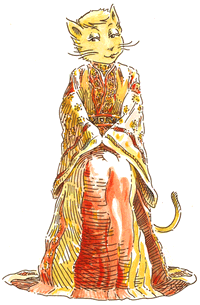
\includegraphics{KTSmeta}
\end{pyglist}

\begin{showresult}
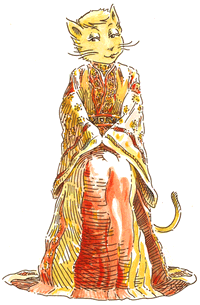
\includegraphics{KTSmeta}
\end{showresult}

이미지 파일이름은 확장자를 빼고 파일 이름만 넣도록 한다. 

하지만 이미지만 달랑 넣기 보다는 \texttt{figure} 환경 안에 사용하기를 권한다.

\begin{pyglist}
\begin{figure}[!hbp]
\centering
\caption{KTS META(Duane Bibby)}
\label{fig:ktsmeta}
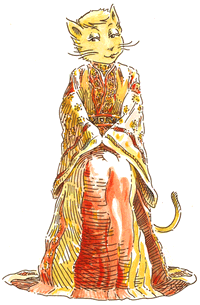
\includegraphics{KTSmeta}
\end{figure}
\end{pyglist}

\begin{figure}[!hbp]
\begin{showresult}
\centering
\caption{KTS META(Duane Bibby)}
\label{fig:ktsmeta}
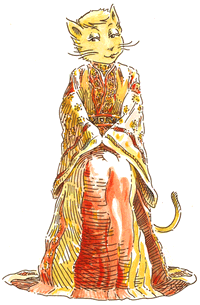
\includegraphics{KTSmeta}
\end{showresult}
\end{figure}

이 명령은 다양한 옵션을 제공하는데 width는 가로, height는 높이, angle은 회전 각도를 뜻한다. 다른 옵션들은 설명서를 참고하라.

여기서 주의할 점은 \verb|\label{}|명령을 사용할 경우, \verb|\caption{}|명령 뒤에 사용해야 한다. 그래야 어딘가에서 \verb|\ref{}|명령으로 내부 참조를 할 때 해당 그림으로 이동할 수 있다.

\begin{pyglist}
\centering
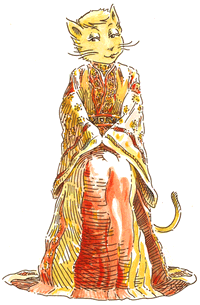
\includegraphics[
	width=0.5\textwidth, 
	height=5cm, 
	angle=15]{KTSmeta}
\end{pyglist}

\begin{showresult}
\centering
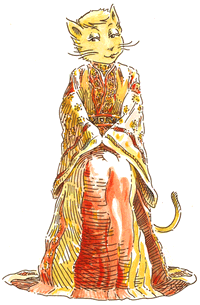
\includegraphics[
	width=0.5\textwidth, 
	height=5cm, 
	angle=15]{KTSmeta}
\end{showresult}

여기서 \verb|0.5\textwidth|는 본문폭(textwidth)의 절반(0.5)을 뜻한다.

\section{xcolor}\label{sec:xcolor}
\index{xcolor}
xcolor 패키지는 색을 다루는 패키지이다. xcolor 패키지가 제공하는 다양한 색상 이름은 물론, 사용자가 직접 색상을 임의로 만들고 이름을 지어줄 수 있다.
\begin{pyglist}
\usepackage[cmyk, dvipsnames, svgnames]{xcolor}
\end{pyglist}
xcolor 패키지를 불러올 때 위와 같이 옵션을 줄 수 있다. cmyk는 색상 모델이다. cmyk는 인쇄할 때 사용하는 색상 모델이다. rgb나 HTML 등의 모델을 사용할 수 있다.

dvipsnames나 svgnames는 미리 정의된 색상이름들을 사용하기 위한 옵션이다. 이들 옵션이 제공하는 색상이름을 바로 사용할 수 있다. 어떤 이름들이 어떤 색상인지를 보려면 xcolor 패키지 설명서를 참고하기 바란다. 내가 좋아하는 HotPink는 svgnames가 제공하는 색상이다.

\begin{pyglist}
나는 \textcolor{HotPink}{핫핑크}가 좋아
\end{pyglist}

\begin{showresult}
나는 \textcolor{HotPink}{핫핑크}가 좋아
\end{showresult}

이제 직접 색상을 만들고 이름을 짓는 방법을 알아보자. \verb|\usepackage{xcolor}|를 한 다음에 아래와 같이 정의한다.

\begin{pyglist}
\definecolor{SunOrange}{cmyk}{0,.47,.78,0}
\end{pyglist}

이 매뉴얼을 여기까지 읽은 사람이라면 이 코드가 어떤 의미인지 알 수 있으리라 생각한다. 다만 마지막에 있는 숫자에 대해서만 간략히 설명하기로 한다. 각 숫자는 Cyan, Magenta, Yellow, Black(Key)에 대한 값이다. RGB가 각각 0부터 255 사이의 값이라면, CMYK는 0부터 1사이의 값이다.

이제 이 색상을 이용해 글자색을 바꿔보자.

\begin{pyglist}
\textcolor{SunOrange}{햇빛오렌지색}
\end{pyglist}

\begin{showresult}
\textcolor{SunOrange}{햇빛오렌지색}
\end{showresult}

\section{mdframed}\label{sec:mdframed}
\index{mdframed}
이 놀라운 패키지는 박스를 꾸밀 때 필요한 모든 기능을 제공한다. 지난 2012년 한국텍학회 학술대회에서 이주호님께서 소개하셨는데, 그 때 만드신 발표자료가 정말 훌륭하다. 나중에 이 패키지의 매뉴얼에도 소개되었다\footnote{\href{http://progress.tistory.com/170}{http://progress.tistory.com/170}}. 이 패키지에 대한 설명은 \href{http://prezi.com/zc355i9tcsgz/talk-kts-2012-mdframed/}{이주호님의 발표자료}를 링크하는 것으로 대신하고, 여기서는 이주호님의 예제코드 중 하나만 보이기로 한다.

이 패키지를 사용하기 위해서는 먼저 아래와 같이 usepackage를 해준다.

\begin{pyglist}
\usepackage[framemethod=tikz]{mdframed}
\end{pyglist}

TikZ\footnote{\href{http://www.texample.net/tikz/}{TikZ 홈페이지}}는 프로그래밍 방식으로 그래픽 요소를 만드는 \TeX 패키지이다. 박스에 멋진 효과를 줄 때 이 TikZ 패키지를  이용해서 만들겠다는 의미이다.

이제 본문에서 mdframed로 박스를 만들어 보자.
\begin{pyglist}
\begin{mdframed}[
	linecolor=Green!80,
	roundcorner=10pt,
	backgroundcolor=Green!10,
	innertopmargin=\topskip,
	frametitleaboveskip=2pt,
	frametitlefont=\bfseries\itshape,
	frametitlerule=true,
	frametitlerulewidth=1pt,
	frametitlebackgroundcolor=Olive!20,
	frametitlealignment=\center,
	leftmargin=1cm,
	rightmargin=1cm,
	frametitle={\normalfont\bfseries\Large%
		\color{DodgerBlue}푸리에 급수의 부분합}]
디리클레는 푸리에 급수의 부분합을 아래와 같이 나타냈습니다.
\[
S_n(x)=\frac{1}{\pi}\int_{\pi}^{\pi}f(t)\frac{sin(n+1/2)(t-x)}{sin(t-x)/2}dt
\]
\end{mdframed}
\end{pyglist}

위 코드의 결과는 다음과 같다.\verbfootnote{수식코드에 쫄지 않아도 된다. 수학자가 아니라면 이렇게 입력할 일이 없고, 수학자라면 이런 수식은 어렵지 않을 것이다.}
\begin{showresult}[innertopmargin=18pt]
\begin{mdframed}[
	linecolor=Green!80,
	roundcorner=10pt,
	backgroundcolor=Green!10,
	innertopmargin=\topskip,
	frametitleaboveskip=2pt,
	frametitlefont=\bfseries\itshape,
	frametitlerule=true,
	frametitlerulewidth=1pt,
	frametitlebackgroundcolor=Olive!20,
	frametitlealignment=\center,
	leftmargin=1cm,
	rightmargin=1cm,
	frametitle={\normalfont\bfseries\Large%
		\color{DodgerBlue}푸리에 급수의 부분합}]
디리클레는 푸리에 급수의 부분합을 아래와 같이 나타냈습니다.
\[
S_n(x)=\frac{1}{\pi}\int_{\pi}^{\pi}f(t)\frac{sin(n+1/2)(t-x)}{sin(t-x)/2}dt
\]
\end{mdframed}
\end{showresult}

%%%
\section{hyperref}\label{sec:hyperref}
\index{hyperref}
문서를 작성하다보면 링크를 만들 경우가 생긴다. 문서 외부의 자료를 참조하는 링크 뿐만 아니라 문서 내에서 참조하는 내부 참조 역시 링크이다. hyperref 패키지는 이런 링크들을 다룬다.

대표적인 명령으로 이런 명령이 있다.

\begin{pyglist}
\href{http://www.ktug.org}{KTUG}
\end{pyglist}

어떻게 사용하는지 쉽게 짐작할 수 있을 것이다. hyperref 패키지는 링크의 색상도 지정할 수 있다. 또한 PDF문서의 속성까지도 지정할 수 있다.

다음은 이 문서에서 사용한 hyperref 패키지 옵션이다.
\begin{pyglist}
\usepackage[
    pdfauthor={dokenzy},
    pdftitle={모두를 위한 LaTeX},
    pdfsubject={LaTeX을 시작하려는 사람들을 위한 성의없는 설명서},
    pdfkeywords={LaTeX, 매뉴얼, 너무 성의없다},
    colorlinks= true,
    linkcolor=blue,
    urlcolor=blue,
    citecolor=blue,
    anchorcolor=blue]{hyperref}
\end{pyglist}

그런데 코드 상에는 아무 문제가 없는데 컴파일 할 때 `! LaTeX Error: Option clash for package hyperref.' 오류가 발생할 수 있다. 사용중인 어느 패키지가 이미 내부적으로 hyperref 패키지를 사용하고 있기 때문이다.\verbfootnote{어떤 패키지가 다른 패키지를 로드할 때는 보통 \verb|\usepackage{}|대신 \verb|RequirePackage{}|명령을 사용한다.} 이럴 때는 hyperref 패키지의 옵션만 설정하자. 프리앰블에서 \verb|\hypersetup{}| 명령으로 설정한다.
\begin{pyglist}
\hypersetup{
    pdfauthor={dokenzy},
    pdftitle={모두를 위한 LaTeX},
    pdfsubject={LaTeX을 시작하려는 사람들을 위한 성의없는 설명서},
    pdfkeywords={LaTeX, 매뉴얼, 너무 성의없다},
    colorlinks= true,
    linkcolor=blue,
    urlcolor=blue,
    citecolor=blue,
    anchorcolor=blue}
\end{pyglist}

\section{tabu}\label{sec:tabu}
\index{tabu}
\LaTeX에서 표를 만드는 것은 손이 많이 가는 작업이다. tabu는 기존의 불편함을 많이 해소하고 괜찮은 인터페이스와 강력한 기능을 제공한다. 이주호님은 \href{http://conf.ktug.org/2011/Welcome.html}{2011년 한국텍학회 학술대회}에서 `표 만들기의 새 표준 tabu'라는 제목으로 이 패키지를 소개해 주셨다. 이 때의 \href{http://conf.ktug.org/2011/Program_files/KTS2011-progress.pdf}{발표자료} 역시 아주 좋은 참고자료이다.

이주호님의 자료가 정말 좋기 때문에 여기서는 이주호님의 발표자료 중 하나만 예를 보이는 것으로 마치겠다.

\begin{pyglist}
\begin{tabu} spread 10pt {X[c]*{3}{|X[2,l]}}
\toprule
$x$ (도) & $\sin x$ & $\cos x$ & $\tan x$ \\
\midrule
\rowfont[c]{\sffamily} 0 & 0 & 1 & 0 \\
1 & 0.0174524 & 0.99984769 & 0.01745506 \\
\rowfont[r]{\large\itshape\bfseries}
2 & 0.03489949 & 0.99939082 & 0.03492076 \\
3 & 0.05233595 & 0.99862953 & 0.05240777 \\
\bottomrule
\end{tabu}
\end{pyglist}

\begin{showresult}
\begin{tabu} spread 10pt {X[c]*{3}{|X[2,l]}}
\toprule
$x$ (도) & $\sin x$ & $\cos x$ & $\tan x$ \\
\midrule
\rowfont[c]{\sffamily} 0 & 0 & 1 & 0 \\
1 & 0.0174524 & 0.99984769 & 0.01745506 \\
\rowfont[r]{\large\itshape\bfseries}
2 & 0.03489949 & 0.99939082 & 0.03492076 \\
3 & 0.05233595 & 0.99862953 & 0.05240777 \\
\bottomrule
\end{tabu}
\end{showresult}
%
\chapter{폰트}\label{chap:font}
\index{font}
\XeLaTeX은 시스템에 설치된 트루타입과 오픈타입 폰트들을 직접 사용할 수 있다. Fontspec 패키지는 이 폰트들을 직관적인 방법으로 사용할 수 있게 해준다. \koTeX 은 내부적으로 Fontspec 패키지를 이용한다. 이주호님이 AJT\footnote{the Asian Journal of TeX}에 쓰신 \href{http://ajt.ktug.org/2010/0401juho.pdf}{Fontspec: \XeTeX의 날개}라는 글은 \XeTeX과 Fontspec 뿐만 아니라 폰트 기술 전반에 대해 정리한 귀한 글이다.\footnote{나는 폰트 기술을 다룬 문서 중에 이보다 좋은 한글문서를 찾지 못했다.}

다양한 폰트들을 보여주려는 특별한 목적이 아니라면 하나의 문서에 3개의 폰트패밀리(font family)를 사용하는 것을 권장한다. 바탕체(serif), 돋움체(sans serif), 타자체(typewriter)가 바로 그것이다. 바탕체는 본문에 쓰이는 기본 폰트, 돋움체는 큰 제목이나 캡션 등에 쓰이는 폰트, 타자체는 그 외 특별한 용도에 쓰인다고 보면 된다.

이들 폰트를 지정하는 방법은 다음과 같다.

\begin{pyglist}
\setmainfont{serif}
\setsansfont{sanserif}
\setmonofont{typewriter}
\setmainhangulfont{바탕글꼴}
\setsanshangulfont{돋움글꼴}
\setmonohangulfont{타자글꼴}
\end{pyglist}

예컨대, 이 문서에 쓰인 한글본문폰트는 다음과 같이 설정했다.
\begin{pyglist}
\setmainhangulfont{HCR Batang LVT}
\end{pyglist}

HCR Batang LVT는 \ref{sec:ktug}\sectionname~\titleref{sec:ktug}에서 언급한 폰트이다. 이 폰트의 이름은 폰트유틸리티 등을 통해 알 수 있다(\figurename~\ref{fig:fontbook1}).

\begin{figure}[!hbtp]
\centering
\caption{서체관리자로 본 함초롬바탕 LVT 폰트}
\label{fig:fontbook1}
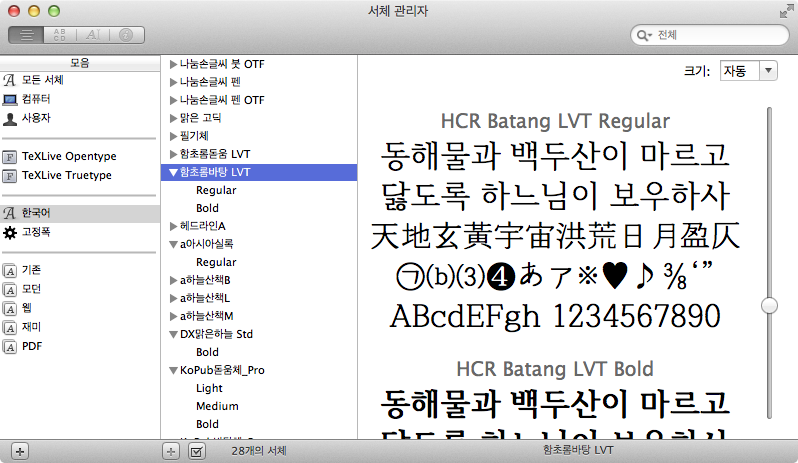
\includegraphics[width=\textwidth]{fontbook1}
\end{figure}

하지만 \figurename~\ref{fig:fontbook2}처럼 이름이 없는 경우도 있다.

\begin{figure}[!hbtp]
\centering
\caption{서체관리자로 본 a아시아실록 폰트}
\label{fig:fontbook2}
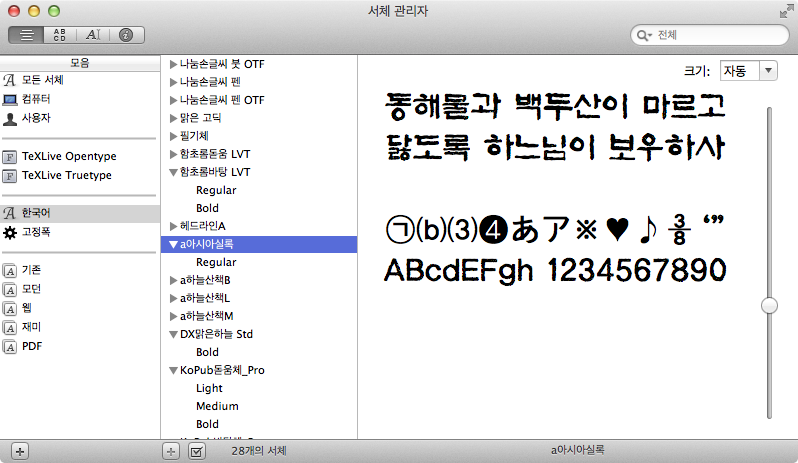
\includegraphics[width=\textwidth]{fontbook2}
\end{figure}

이런 경우에는 다음과 같이 폰트의 파일명으로 지정할 수 있다.\footnote{폰트파일명이 한글인 경우 안될 수 있다. 그럴 때는 파일명을 영문자로 바꾸자. 자세한 내용은 \texttt{oblivoir-simpledoc.pdf}의 5.5절 ExternalLacation을 살펴보라.}
\begin{pyglist}
\setsanshangulfont{a아시아실록.otf}
\end{pyglist}

영문폰트와 한글폰트를 따로 지정하는 이유는, 한글폰트에 들어있는 영문폰트가 영어권 회사의 폰트보다 좋지 않기 때문이다. 따라서 한글폰트와 잘 어울리는 영문폰트를 선택하는 것이 중요하다. 무슨 폰트를 써야할지 막막한 사람은 이주호님이 문서작성워크숍에서 발표한 자료(\href{http://wiki.ktug.org/wiki/wiki.php/LaTeXWorkshop/2013?action=download&value=talk1_typography_by_progress.pdf}{타이포그래피})를 참고하자.

\chapter{Minimal Working Example}\label{chap:mme}
\index{Minimal Working Example}
이제 \LaTeX으로 많은 것들을 할 수 있을 것이다. 차례, 상호참조, 목록, 박스꾸미기, \tablename, \ldots~하지만 컴파일하다가 오류를 만난 확률도 그만큼 높아질 것이다. 이제 어떻게 하면 오류를 찾고 해결할 수 있는지 그 방법을 찾아보자.

대부분의 오류는 다음과 같은 경우에 발생한다.

\begin{itemize}
\item 오타
\item 괄호의 짝이 맞지 않을 때
\item \verb|\begin{}|, \verb|\end{}| 짝이 맞지 않을 때
\item 없는 명령을 사용했을 때
\item 없는 환경을 사용했을 때
\item 옵션을 잘못 사용했을 때
\end{itemize}

단순한 명령과 환경만으로 만든 텍 문서에서 오류를 해결하는 방법은 그리 어렵지 않다. 하지만 많은 패키지를 쓰고 직접 명령이나 환경을 정의해서 사용하는 큰 규모의 문서라면 오류를 찾는 것 자체가 어려울 것이다. 다행히 \LaTeX은 컴파일시 발생하는 오류에 대해 꽤 정확하게 알려준다. 컴파일 중에 오류가 발생하면 먼저 오류 메시지를 잘 읽어보자.

오류메시지를 잘 읽어보면 어느 부분에서 오류가 발생했는지 알 수 있다. 이 오류메시지가 아주 정확한 경우도 있지만 그렇지 않은 경우도 있다. 어떤 부분의 오류 때문에 다른 부분이 오류가 발생하는 경우이다. 이런 오류는 원인을 알아내는 것이 어려울 수 있다. 패키지가 서로 충돌하는 경우도 어렵다. 하지만 Minimal Working Example(MWE)을 만들어보면 이런 경우도 오류의 원인을 비교적 쉽게 찾아낼 수 있다. 이 \chaptername의 목표는 오류의 원인을 찾는 것이지 오류를 해결하는 방법을 찾는 것이 아니다.

\section{왜 MWE를 만들어야 하는가?}\label{sec:mme}
문서를 만들다보면 이런저런 명령과 환경을 쓰기 위해 패키지를 사용하기 마련이다. 그러다가 에러메시지만으로 오류의 원인을 찾을 수 없게 되면 곤란해진다.\footnote{제일 곤란한 것은 오류없이 컴파일은 되는데 원하지 않은 결과가 나오는 것이다.} MWE는 바로 그런 경우에 특히 유용하다. 먼저 현재의 파일을 복사(\texttt{foo-mwe.tex})한다. 복사한 파일에서 오류와 관련없는 부분을 조금씩 삭제하면서 컴파일을 해본다. 이렇게 하다보면 원래 문서에서 발생한 오류과 같은 오류를 갖는 최소한의 텍 코드를 만들게 된다. 비록 컴파일할 때 오류가 발생하지만 어떤 환경(엔진, 클래스, 패키지, 명령, 인코딩 등 많은 조건들)에서 그런 오류가 발생하는지 알 수 있다.

이 문서를 작성하면서 의도한대로 결과가 나오지 않아 몇 번의 MWE를 만들어야 했다. 가장 최근에 만든 MWE 작업과정을 예로 들어보이겠다.

그림의 캡션 모양을 수정하기 위해 프리앰블에 다음과 같은 코드를 입력했다. 하지만 결과가 바뀌지 않았다.
\begin{pyglist}
\captiondelim{ }
\captionnamefont{\footnotesize\bfseries\sffamily}
\captiontitlefont{\footnotesize\sffamily}
\end{pyglist}
50페이지 분량의 컴파일 과정이 후다닥 지나가 버린다. \texttt{log}파일도 2500줄이 넘는다. MWE를 만들어야겠다.

\begin{enumerate}
\item \texttt{latex4all.tex}파일을 \texttt{captiontest.tex}파일로 복사한다.
\item 그림 캡션이 의도한대로 잘 나오는지 확인만 하면 되니까 첫번째 그림부분을 제외하고 본문에서 내용을 전부 삭제한다\verbfootnote{당연히 문서 맨 끝에 \verb|\end{document}|는 있어야한다.}.
\item 프리앰블에서도 그림과 상관없는 것들을 모두 지운다.
\item 이제 의도한대로 잘 나온다. 프리앰블에 뭔가 잘못된 것이 있을 것이다.
\item 그림 캡션과 관련이 있을테니 이와 관련된 패키지를 찾아봐야겠다.
\item \verb|\usepackage{caption}|이 있다. 이걸 다시 넣고 테스트해보자.
\end{enumerate}

이런 경고가 보인다.

\begin{pyglist}
Class memoir Warning: You are using the caption package with
the memoir class. To prepare we will now reset all captioning
macros and configurations to kernel defaults, and then let the
caption package take over. Please remember to use the caption
package interfaces in order to configure your captions.
\end{pyglist}

그렇다. 내가 사용하는 \texttt{oblivoir}라는 클래스는 \texttt{memoir}클래스 위에서 동작하는데, \texttt{memoir}클래스에서 제공하는 캡션 관련 명령들이 \texttt{caption} 패키지 때문에 동작하지 않은 것이었다. 

물론 이 경고 메시지는 1,000줄 짜리 \texttt{latex4all.tex}파일을 컴파일 할 때도 있었다. 하지만 2,500줄이 넘는 \texttt{log}파일에서 이걸 찾아내려면\ldots

이제 원인을 알았으므로 문제를 해결해보자. 다행히 이 문제는 \verb|\usepackage{caption}|을 지우는 것으로 해결할 수 있었다. 하지만 어떤 경우엔 해결방법을 찾는 것이 어려울 때도 있는 법, 이럴 때 해결하는 방법은
\begin{inparaenum}[1)]
\item 구글이나 KTUG에서 검색하거나, \item KTUG에 질문하는 것이다.
\end{inparaenum}

검색은 직접 해보면 되고, 이 문서에서는 KTUG에 질문을 올리는 요령을 간략히 설명한다.

\begin{enumerate}
\item MWE를 만든다.
\item 그림파일이 있다면 그림파일도 포함한다.
\item KTUG의 질문게시판에 자신의 텍 환경(운영체제, TeXLive 버전, 사용한 텍 엔진 등)과 오류내용, 원하는 결과 등을 적고
\item 파일을 첨부해서 올린다. 압축포맷은 \texttt{zip}이 가장 좋다.
\end{enumerate}

`이 정도면 되겠지?'하고 위아래 싹뚝 자르고 코드 일부만 올리고 질문하는 분들이 있다. 또는 아무 코드 없이 얘기만 하는 분들도 있다. 이렇게 올리면 대답도 추상적일 수 밖에 없다. MWE파일을 만들어서 올리자. 이것이 서로 편한 길이다.

텍 코드에는 오류가 없는데도 컴파일 중에 오류가 발생할 수 있다. 텍은 컴파일을 하면서 몇 가지 부수파일들을 만드는데 이런 부수파일 때문에 오류가 발생할 수 있다. \texworks에서는 [메뉴]-[부수파일 삭제]를 통해 쉽게 지울 수 있다. 웹브라우저에서 캐쉬를 지우는 것과 비슷하다. 

\section{경고(WARNING) 다루기}
\index{경고}
\index{WARNING}
컴파일을 하면 경고가 발생하는 것을 쉽게 볼 수 있다. 특히 \texttt{Overfull} 오류를 자주 볼 수 있다. 이 경고는 내용 일부가 본문 너비보다 넓은 경우에 발생한다. 어떤 경고는 무시해도 되고 어떤 경고는 고쳐야 하는 경우도 있다. 판단은 각자 알아서 잘 한다.

폰트때문에 경고가 발생하는 경우도 있다.\footnote{이 문서를 작성할 때 발생한 경고인데 나는 무시하기로 했다.}
\begin{pyglist}
** WARNING ** Unrecognized OpenType/TrueType cmap format.
** WARNING ** Unable to read OpenType/TrueType Unicode cmap table.
** WARNING ** Failed to load ToUnicode CMap for font "AppleSymbols"
\end{pyglist}
대부분 폰트 문제이다. 좋은 폰트는 이런 경고가 없다. 그래서 폰트를 잘 골라써야 한다.

상호참조에 문제가 있어도 경고가 발생한다. 다음은 이 문서를 컴파일하는 중에 나온 경고이다.
\begin{pyglist}
LaTeX Warning: Reference `chap:xcolor' on page 31 undefined on input line 766.
\end{pyglist}
\verb|\label{sec:xcolor}|라고 라벨을 붙였는데, 참조할 때는 \verb|\ref{chap:xcolor}|라고 해서 발생한 경고이다.

코드에 아무런 문제가 없어도 상호참조 경고가 발생할 수 있다.
\begin{pyglist}
LaTeX Warning: Label(s) may have changed. Rerun to get cross-references right.
\end{pyglist}
이 경고는 텍 파일에 오류는 없지만 참조하는 라벨이 해당 위치에 없는 경우 발생한다. 예를 들면 내용이 변경되면서 쪽번호나 장절번호가 바뀔 수 있는데 이것이 반영이 아직 안됐을 때 발생한다. 해결하는 방법은 한 번 더 컴파일해주면 된다. 만약 해결하지 않으면 쪽번호가 나와야 할 곳이 `?'로 나오게 된다.
%
\chapter[한국어문서 조판하기]{\koTeX과 oblivoir로 한국어문서 조판하기)}\label{chap:kotex}
\ref{chap:essential}\chaptername~\titleref{chap:essential}까지만 배워도 꽤 멋진 문서를 만들 수 있다. 하지만 한국어 문서를 작성하기 위해서는 여기서 소개하는 \koTeX\을 배울 필요가 있다. \koTeX\은 단순히 한글 입출력에 그치지 않고 `한국어 문서 조판'을 하기 위한 많은 기능들을 제공한다. \koTeX은 매우 많은 기능을 제공하기 때문에 내가 다 알지 못한다. 여기서는 이런 기능들이 있다는 소개만 간략히 한다.

\section{\koTeX}
\index{koTeX}
영어권에서 만들어진 \TeX을 이용해서 한글을 조판하기 위해서 많은 노력들이 있었고, 그 결과 현재의 \koTeX~v2.0이 만들어졌다. \koTeX은 다음의 패키지들을 총칭한다.

\begin{description}
\item[\koTeX-utf] legacy TeX엔진에 대응하는 패키지
\item[cjk-\ko] CJK패키지(개발자 Werner Lemberg)를 이용하여 유니코드 한글을 식자하는 패키지
\item[\XeTeX-\ko] \XeTeX 엔진에 대응하는 한글 식자 패키지 
\item[\LuaTeX-\ko] \LuaTeX 엔진에 대응하는 한글 식자 패키지 
\item[oblivoir] memoir클래스를 이용한 한글 문서 작성 클래스와 패키지 묶음\footnote{이 문서는 이 클래스로 만들어졌다.}
\item[\koTeX 유틸리티] 한글 문서 작성에 필요한 유틸리티들
\end{description}

어려울 수 있지만 어렵지 않게 쓸 수 있다. \textbf{우리는 그냥 이렇게만 하면 된다}.
\begin{pyglist}
\usepackage{kotex}
\end{pyglist}
위와 같이 선언하면 \koTeX패키지가 알아서 필요한 패키지를 불러온다. 예를 들어, 텍 엔진이 \XeLaTeX이면 \XeTeX-\ko패키지를 불러온다. 만약 텍 엔진이 \LuaLaTeX이라면 \LuaTeX-\ko 패키지를 불러온다. 즉, \koTeX 패키지가 하는 일은 텍 엔진에 따라 필요한 패키지를 자동으로 호출하는 것이다.

\koTeX이 제공하는 기능들을 나열해보면,
\begin{itemize}
\item 우리말 이름(장, 절, 차례, 등)
\item \dotemph{방점}, \useremph[10pt]{\tiny★}{이런 방점까지!}
\item 한글식 카운터: \jaso{hindex}, \pjaso{hindex}, \ojaso{hindex}, \gana{hindex}, \ogana{hindex}, \pgana{hindex}, \onum{hindex}, \pnum{hindex}, \oeng{hindex}, \peng{hindex}, \hnum{hindex},\Hnum{hindex}, \hroman{hindex}, \hRoman{hindex}
\item 자동조사
\item 미세조정(자간, 어간, 행간, 행 나눔, 수식과의 간격 등)
\item 한글 책갈피, 찾아보기, 참고문헌 등
\item 옛한글
\item 한글문서 서식
\item 세로쓰기
\end{itemize}

자세한 내용은 \ko.\TeX설명서를 읽어보기 바란다. 여기서는 세로쓰기의 예만 간략히 보이겠다.

\begin{figure}[!hbtp]
\begin{center}
\begin{vertical}{11em}
\hangulfontspec[ Vertical=RotatedGlyphs]{a아시아실록.otf}
\noindent{\Large 나는 우리나라가 세계에서 가장 아름다운 나라가 되기를 원한다. 가장 부강한 나라가 되기를 원하는 것은 아니다. 내가 남의 침략에 가슴이 아팠으니, 내 나라가 남을 침략하는 것을 원치 아니한다. 우리의 부력은 우리의 생활을 풍족히 할 만하고, 우리의 강력은 남의 침략을 막을 만하면 족하다. 오직 한없이 가지고 싶은 것은 높은 문화의 힘이다.}
\end{vertical}
\caption*{`내가 원하는 우리나라(백범 김구)' 중 일부}
\end{center}
\end{figure}

\section{oblivoir 클래스}\label{sec:oblivoir}
\index{oblivoir}
\koTeX을 이용하면 아름다운 한국어 문서를 조판할 수 있다. 그러기 위해서는 다양한 옵션들을 잘 활용해야 한다. 하지만 나처럼 전문가가 아닌 사람은 원하는 게 무엇인지 조차 잘 모를 수 있다. 옵션을 주어도 제대로 쓸 줄을 모른다.

oblivoir는 바로 그런 사람들이 좋아할 만한 클래스이다. memoir 클래스\footnote{많은 기능을 내장한 클래스. 한글로 번역된 문서}에 \koTeX을 내장한 이 클래스는 한국어 문서 조판을 위한 설정이 잘 되어 있다. 따라서 \koTeX패키지를 따로 불러들이지 않아도 된다. 이 문서 역시 oblivoir를 사용한다.

따라서 대부분의 한국사람에게 가장 적절한 한국어 문서 제작 방법은 oblivoir클래스를 이용하는 것이다. oblivoir 역시 좋은 설명서가 있으니 그것을 참고하도록 하자. \texttt{<texdoc oblivoir>}
%%%%
\chapter{좀 더 \LaTeX스럽게}\label{intermediate}
지금까지 \LaTeX과 \koTeX의 기본 명령들을 살펴봤다. 하지만 \LaTeX이 강력한 이유는 그 자체로 하나의 언어이기 때문에 사용자가 직접 명령이나 환경을 만들어 쓸 수 있다는 것이다.
\section{사용자 정의 명령}\label{sec:newcommand}
지금까지는 클래스나 패키지가 제공하는 명령만 사용했다. 이제 직접 명령을 만들어보자.

\subsection{가장 간단한 명령}
\index{newcommand}
만약 C++언어를 만든 비야네 스트롭스트룹(Bjarne Stroustrup)에 대해 글을 쓴다고 하자. 당연히 이 사람의 이름이 자주 쓰일 것이다. 그런데 철자가 길고 어렵다. 뿐만 아니라 영어로 표기할지 한글로 표기할지도 결정하지 못했다. \LaTeX에서는 아무 문제가 안된다.
\begin{pyglist}
...
\newcommand{\bjarne}{Bjarne Stroustrup}
...
\begin{document}
\bjarne
...
\end{pyglist}

\verb|\newcommand|~명령은 새 명령을 정의하는 명령이다.
\newcommand{\bjarne}{Bjarne Stroustrup}

\begin{showresult}
\bjarne
\end{showresult}

만약에 이름을 한글로 바꾸어야 한다면
\begin{pyglist}
\newcommand{\bjarne}{비야네 스트롭스트룹}
\end{pyglist}
으로 선언하면 된다. 이제 본문에서 \verb|\bjarne|라고 쓴 곳은 전부 `비야네 스트롭스트룹'이라고 나올 것이다.

\subsection{옵션이 있는 명령}
\label{subsec:cmd_with_option}
\ref{sec:xcolor}\chaptername~\titleref{sec:xcolor}의 예제에서 다음과 같은 명령을 사용했다.
\begin{pyglist}
\textcolor{SunOrange}{햇빛오렌지색}
\end{pyglist}

햇빛오렌지색을 자주 사용한다면 좀 더 간편한 방법을 찾아보자.

\begin{pyglist}
\newcommand{\sunge}[1]{\textcolor{SunOrange}{#1}}
\sunge{간편하게 쓰는 햇빛오렌지색}
\end{pyglist}

\newcommand{\sunge}[1]{\textcolor{SunOrange}{#1}}
\begin{showresult}
\sunge{간편하게 쓰는 햇빛오렌지색}
\end{showresult}

\subsection{옵션에 기본값을 주는 명령}
방금 전처럼 하면 항상 \sunge{햇빛오렌지색}만 쓸 수 있다. 만약 다른 색상을 쓰고 싶다면 저런 명령을 색상마다 만들어야 할까? 제일 좋은 방법은 \sunge{햇빛오렌지색}을 기본값으로 주고, 다른 색상을 쓰고 싶을 때만 색상을 지정해 주는 것이다.

\begin{pyglist}
\newcommand{\sunnytext}[2][SunOrange]{\textcolor{#1}{#2}}
기본색은 \sunnytext{햇빛오렌지색}이지만,
다른색도 \sunnytext[Goldenrod]{Goldenrod색}도 할 수 있어요.
\end{pyglist}

\newcommand{\sunnytext}[2][SunOrange]{\textcolor{#1}{#2}}

\begin{showresult}
기본색은 \sunnytext{햇빛오렌지색}이지만,
다른색도 \sunnytext[Goldenrod]{Goldenrod색}도 할 수 있어요.
\end{showresult}

결과적으로 \verb|\textcolor{}{}|명령과 별반 다르지 않게 됐지만, 이런 식으로 인자와 옵션이 들어가는 명령을 만들 수 있다는 예시로는 괜찮다고 생각한다.
\subsection{renewcommand}
이미 사용중인 명령(그 명령이 클래스에서 제공하든, 패키지가 제공하든, 직접 정의한 것이든)을 다시 정의해야 할 경우가 생기면 \verb|\renewcommand|명령을 사용한다. 이 명령은 사용자 정의 명령보다는 클래스나 패키지가 제공하는 명령을 수정해야 할 경우에 많이 사용된다. 클래스나 패키지를 직접 수정하는 것은 절대 하지 않기를 바란다. 대신 \verb|renewcommand|를 사용하여 다시 정의하도록 하자. 사용방법은 \verb|\newcommand{}|와 같다.

\section{사용자 정의 환경}
\index{newenvironment}
\verb|\newenvironment{}|명령으로 사용자 정의 환경을 만들 수 있다.

다음은 lshort-kr문서에 나온 예제이다.

\begin{pyglist}
\newenvironment{king}
	{\rule{1ex}{1ex}%
		\hspace{\stretch{1}}}
	{\hspace{\stretch{1}}%
      \rule{1ex}{1ex}}
\begin{king}
My humble subjects \ldots
\end{king}
\end{pyglist}
\newenvironment{king}
	{\rule{1ex}{1ex}%
		\hspace{\stretch{1}}}
	{\hspace{\stretch{1}}%
      \rule{1ex}{1ex}}

\begin{showresult}
\begin{king}
My humble subjects \ldots
\end{king}
\end{showresult}

\section{파일 나누기}
\index{파일 나누기}
\LaTeX의 가장 큰 장점 중 하나는 파일을 분리하여 관리할 수 있다는 점이다. 대규모 문서, 또는 공동으로 문서를 작성할 때 특히 유용하다.
\begin{pyglist}
\include{filename}
\end{pyglist}
이 명령은 filename을 현재 tex 파일에 삽입한다. 이 때 호출된 페이지는 새 페이지에서 시작하게 된다.\verbfootnote{내부적으로 \verb|\clearpage| 명령이 호출되기 때문이다.}

\begin{pyglist}
\includeonly{file1, file2, file3}
\end{pyglist}
이 명령은 프리앰블에서만 쓸 수 있다. \verb|\include{}|명령을 사용할 때 여기에 열거된 파일들만 삽입할 수 있다.

만약 다른 파일을 삽입할 때 새 페이지로 시작하는 것이 싫으면 \verb|\include{filename}| 대신 \verb|\input{filename}| 명령을 사용하자.
%%%%
\chapter{추천 문서}\label{chap:docs}
내가 이 문서를 쓰기까지 많은 자료를 공부하고 참고했다. 꼼꼼히 읽은 문서도 있고 어려워서 잘 모르고 넘어간 문서도 있다. 한 번 읽고 넘어간 문서도 있고 몇 번이고 본 문서도 있다. `클래스 oblivoir와 책 만들기'같은 내 수준에는 어려운 문서도 있고, Donald Knuth교수의 일화가 실린 재밌는 문서도 있다. 본문에 소개된 문서도 있고 그렇지 않은 문서도 있다. \LaTeX을 써보고 싶은 사람이라면 필수 매뉴얼 정도는 정독하길 바란다.

\section{\LaTeX 초보자를 위한 필수 매뉴얼}
\begin{description}
\item[lshort-kr] \LaTeX 전반에 대해 상세하게 다루는 문서
\item[kotexdoc] \koTeX 전반에 대해 상세하게 다루는 문서.
\item[xetexko-doc] \koTeX중 \XeTeX-\ko에 대해 다루는 문서.
\end{description}

\section{\LaTeX을 더 알고 싶은 사람을 위한 글}
한국텍학회에서는 `\href{ajt.ktug.or.kr}{The Asian Journal of TeX}'이라는 학술지를 통해 텍을 이용한 조판 및 인쇄 기술 전반에 대해 많은 논문을 발표했다. 여기 실린 모든 글들이 훌륭하지만 \koTeX 및 \XeLaTeX과 밀접한 글 몇 가지만 소개를 한다.
\begin{description}
\item[\href{http://ajt.ktug.org/2011/0501karnes.pdf}{클래스 oblivoir와 책 만들기}] 김강수
\item[\href{http://ajt.ktug.org/2009/0301karnes.pdf}{한글 텍 : 과거, 현재, 그리고 미래}] 김강수
\item[\href{http://ajt.ktug.org/2010/0401juho.pdf}{Fontspec: \XeTeX의 날개}] 이주호
\item[\href{http://ajt.ktug.org/2007/0102khlee.pdf}{Oblivoir를 이용한 문서 작성}] 이기황
\end{description}

\section{그 외 참고할만한 글}
\begin{description}
\item[\href{http://wiki.ktug.org/wiki/wiki.php/MemucsManual?action=download\&value=memucs-manual.pdf}{Memucs Manual}] 김강수 옮김
\item[\href{http://faq.ktug.org/wiki/uploads/DonaldKnuth.pdf}{한없이 다양한 분야에 걸린 관심, 하나의 공통된 맥락}] 데니스 샤샤, 캐시 레이저어, 박영숙 옮김\footnote{세종연구원에서 출간된 `컴퓨터를 만든 15인의 과학자(Out of their minds)' 중 Donald Knuth 편}
\item[\href{http://faq.ktug.org/faq/SampleDocument?action=download&value=LaTeXStance200912.pdf}{레이텍을 빨리 쓸 수 있는 방법 2009}] 이호재
\item[\href{http://faq.ktug.org/faq/Karnes/2010-09?action=download&value=latex4wp-ko-7.pdf}{워드 프로세서 사용자를 위한 \LaTeX}] 김강수 옮김
\item[\href{http://faq.ktug.org/faq/LaTeXWorkshop/2010?action=download&value=LaTeXLectNotes.pdf}{라텍 소개 및 기본 사용방법}] 조진환
\item[\href{http://faq.ktug.org/faq/LaTeXWorkshop/2010?action=download&value=Introduction_to_Digital_Typography.pdf}{Introduction to
Digital Typography}] 조진환
\item[\href{http://faq.ktug.org/faq/LaTeXWorkshop/2009?action=download&value=WS2009-a.pdf}{\XeLaTeX 문서작성의 실제}] 김강수
\item[\href{http://faq.ktug.org/faq/LaTeXWorkshop/2008Spring?action=download&value=commands.pdf}{스타일 작성을 위한 명령어 모음}] 2008년 공주대 워크숍 강좌팀
\item[\href{http://progress.tistory.com/attachment/ik2.pdf}{article 클래스를 파헤쳐보자}] 2008년 공주대 워크숍 강좌팀
\item[\href{http://faq.ktug.org/faq/LaTeXWorkshop/2008Spring?action=download&value=listandparagraph.pdf}{문단과 리스트}] 김강수
\item[\href{http://faq.ktug.org/faq/LaTeXWorkshop/SS081128?action=download&value=SSWS.pdf}{\LaTeX 활용하기}] 김강수
\end{description}
%%%
\clearpage
\printindex

\pagestyle{empty}
\pagenumbering{gobble}
\chapter*{마치며}
근본없는 \LaTeX 매뉴얼은 여기까지다. 힘들어서 맞춤법 수정도 포기했다. tex 소스가 겨우 1050줄에 불과한, A4기준 50쪽도 안되는 문서인데도 불구하고 힘들다. memoir설명서나 lshort-kr같은 문서를 번역하신 분들의 노고가 새삼 더 크게 느껴진다.

영국이나 미국 등에서 초등학생부터 컴퓨터 프로그래밍 교육을 시작한다고 한다. 특히 영국은 5세부터는 간단한 프로그래밍 과정을 가르치고, 11세 이상 학생에게는 실제 프로그래밍 언어를 교육한다고 한다. 나는 \LaTeX 교육도 프로그래밍 교육 이상의 효과가 있을 것이라고 생각한다. 프로그래밍하듯이 글쓰기를 하니 이보다 좋은 교육방법이 있을까? 또한 웹퍼블리셔에게도 좋은 훈련 방법이 될 것이다. validator만 통과한다고 좋은 마크업이 아니잖은가.

\vfill
\begin{flushright}
\zapfino{Dokenzy}
\end{flushright}

%
\renewcommand\appendixname{부록}
\AttachAppendixTitleToSecnum
\AppendixTitleToToc
\appendix
\section{이 문서를 컴파일하는 방법}

이 문서를 컴파일하려면 다음과 같은 것이 필요하다.
\begin{enumerate}[(1)]
\item python pygments.\footnote{\url{http://pygments.org/}}
python과 setuptools가 설치되어 있으면 다음과 같이 설치한다.
\begin{verbatim}
$ pip install pygments
\end{verbatim}
\item a아시아실록 폰트. 아시아 폰트의 폰트통\footnote{\url{http://www.asiafont.com/asia2009/asia_menu_fonttong.php}}을 이용하여 설치한다.
\item arara-rules-ko 패키지. 이것은 KTUG 사설저장소\footnote{\url{http://wiki.ktug.org/wiki/wiki.php/KtugPrivateRepository}}를 통하여 다음과 같이 설치한다.
\begin{verbatim}
$ tlmgr install arara-rules-ko
\end{verbatim}
\end{enumerate}

컴파일은 arara로 한다. arara는 \TeX\,Live에 들어 있다.
\begin{verbatim}
$ arara latex4all
\end{verbatim}
\clearpage

\printindex

\pagestyle{empty}
\pagenumbering{gobble}
\chapter*{마치며}
근본없는 \LaTeX 매뉴얼은 여기까지다. 힘들어서 맞춤법 수정도 포기했다. tex 소스가 겨우 1050줄에 불과한, A4기준 50쪽도 안되는 문서인데도 불구하고 힘들다. memoir설명서나 lshort-kr같은 문서를 번역하신 분들의 노고가 새삼 더 크게 느껴진다.

영국이나 미국 등에서 초등학생부터 컴퓨터 프로그래밍 교육을 시작한다고 한다. 특히 영국은 5세부터는 간단한 프로그래밍 과정을 가르치고, 11세 이상 학생에게는 실제 프로그래밍 언어를 교육한다고 한다. 나는 \LaTeX 교육도 프로그래밍 교육 이상의 효과가 있을 것이라고 생각한다. 프로그래밍하듯이 글쓰기를 하니 이보다 좋은 교육방법이 있을까? 또한 웹퍼블리셔에게도 좋은 훈련 방법이 될 것이다. validator만 통과한다고 좋은 마크업이 아니잖은가.

\vfill
\begin{flushright}
\zapfino{Dokenzy}
\end{flushright}

\end{document} 
